%==============================================================================
\chapter{Model emulation, parameter fitting and uncertainty 
quantification}\label{cha:chapter3}
%==============================================================================
%
%
%
\begin{remark}{Outline}
    In this chapter, we present the principal tools to model emulation, fitting and uncertainty quantification.
\end{remark}


%
%
%
\section{Model input parameters}
The presented full rat heart contraction model is regulated by $71$, $17$, $18$ parameters for respectively the ionic, cell contraction, tissue $+$ boundary components. We selected specific parameters as representative regulators of each of these sub-models, for a total of $8$ parameters. Specifically, $2$ parameters ($\Caif$, $\koff$) described the thin filament kinetics, $2$ parameters ($\kxb$, $\tref$) described the thick filament kinetics, and $4$ parameters ($\p$, $\pao$, $\Z$, $\Cone$) described boundary conditions and tissue properties. The $8$ parameters considered are described in Table~\ref{tab:paramswithdef}. A fixed calcium transient simulated using the adopted ionic model was used as electrical stimulus for the whole heart activation.

\begin{table}[!ht]
    \myfloatalign
    \begin{tabularx}{\textwidth}{llX}
    \toprule
    \tableheadline{Parameter} & \tableheadline{Units}                   & \tableheadline{Definition} \\
    \midrule
    $\Caif$                   & $\SI{}{\micro\Molar\tothe{1-1/\ntrpn}}$ & reference $\Ca$ thin filament sensitivity \\
    $\koff$                   & $\SI{}{\per\milli\second}$              & unbinding rate of $\Ca$ from TnC \\
    $\kxb$                    & $\SI{}{\per\milli\second}$              & cross-bridges cycling rate \\
    $\tref$                   & $\SI{}{\kilo\pascal}$                   & maximal reference tension \\
    $\p$                      & $\SI{}{\kilo\pascal}$                   & end-diastolic pressure \\
    $\pao$                    & $\SI{}{\kilo\pascal}$                   & aortic systolic pressure \\
    $\Z$                      & $\SI{}{\mmHg\second\per\milli\liter}$   & aortic characteristic impedance \\
    $\Cone$                   & $\SI{}{kPa}$                            & tissue stiffness \\
    \bottomrule
    \end{tabularx}
    \caption{Model parameters and their definitions}
    \label{tab:paramswithdef}
\end{table}


%
%
%
\section{Model output features}
We are interested in characterising the LV contractile function in the rat models A typical full rat heart contraction mechanics model's output consists in LV volume and pressure transients, along with the corresponding \textit{pressure-volume} (\acs{PV}) \textit{loop}. Multiple-beats simulations are commonly run to reach a more stable \enquote{limit cycle}, and only the last-beat's curves are analysed. In Figure~\ref{fig:examplepvloop}, an example $4$-beat simulation is shown with the limit cycle curves highlighted.

\begin{figure}[!ht]
    \myfloatalign
    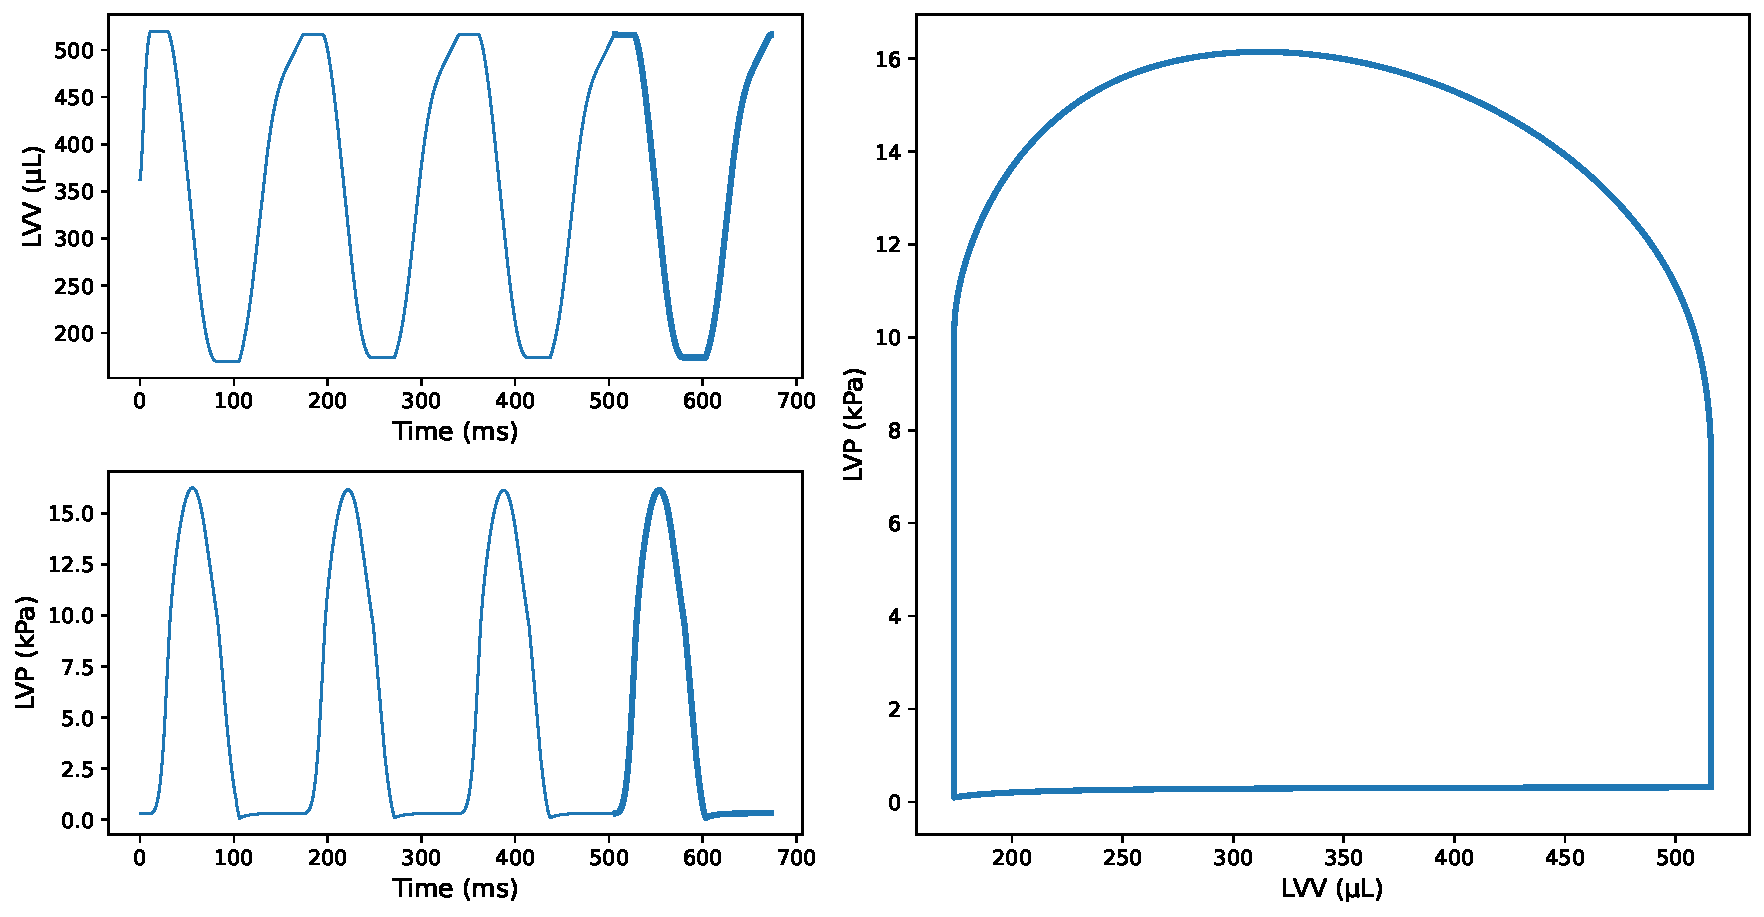
\includegraphics[width=\textwidth]{figures/chapter03/a_typical_model_output.pdf}
    \caption{Rat heart contraction mechanics model $4$-beat simulation output. LV volume and pressure transients are drawn in a thin blue line, and their last-beat's tracts, along with the corresponding PV loop, are drawn in a thick blue line.}
    \label{fig:examplepvloop}
\end{figure}

\vspace{0.2cm}
To quantitatively characterise the LV activity, we extracted from the last-beat's curves $12$ scalar features of interest which are commonly used to characterise LV systolic and diastolic functions:
%
\begin{align}
    &\text{EDV}= \max_{t>0}{v_{\textrm{LV}}(t)} \\
    &\text{ESV}= \min_{t>0}{v_{\textrm{LV}}(t)} \\
    &\text{EF}= 100\times\frac{\text{EDV}-\text{ESV}}{\text{EDV}} \\
    &\text{IVCT}= t_1-t_0 \\
    &\text{ET}= t_2-t_1 \\
    &\text{IVRT}= t_3-t_2 \\
    &\text{Tdiast}= t_4-t_2 \\
    &\text{PeakP}= \max_{t>0}{p_{\textrm{LV}}(t)} = p_{\textrm{LV}}(t_5) \\
    &\text{Tpeak}= \argmax_{t>0}{p_{\textrm{LV}}(t)} = t_5 \\
    &\text{ESP}= p_{\textrm{LV}}(t_2) \\
    &\text{maxdP}= \max_{t>0}{\frac{dp_{\textrm{LV}}(t)}{dt}} \\
    &\text{mindP}= \min_{t>t_2}{\frac{dp_{\textrm{LV}}(t)}{dt}}
\end{align}

\noindent
where

\vspace{0.2cm}
\begin{tabular}{ll}
    $t_i,\,\text{for}\,\,i=0,\,\dots,\,5$ & positive time points (explained in Figure~\ref{fig:lvfeatsextraction}) \\
    $v_{\textrm{LV}}(t)$ & LV volume transient \\
    $p_{\textrm{LV}}(t)$ & LV pressure transient
\end{tabular}

\vspace{0.3cm}\noindent
The process of LV output features extraction is illustrated in Figure~\ref{fig:lvfeatsextraction}, and all the features definition are provided in Table~\ref{tab:lvfeatures}.

\begin{figure}[!ht]
    \myfloatalign
    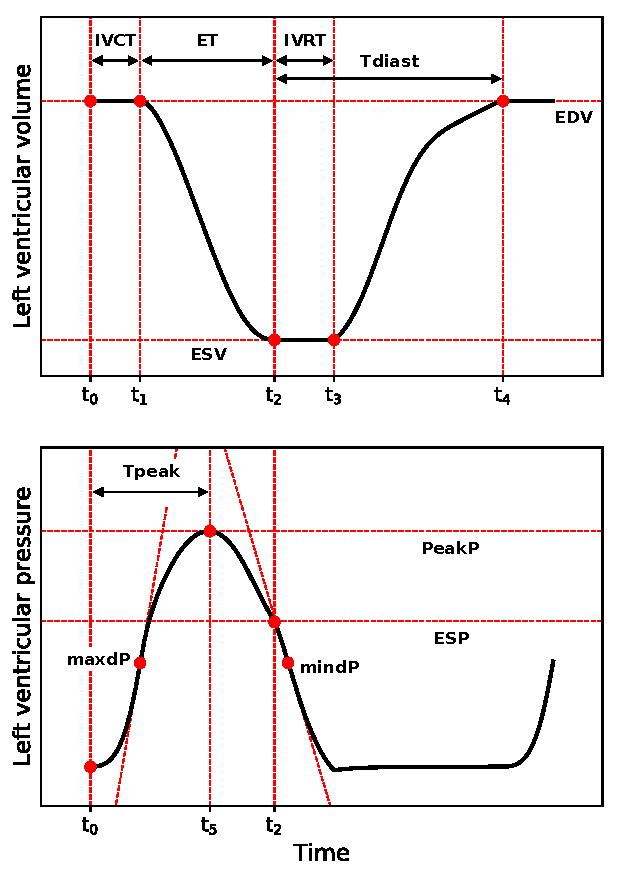
\includegraphics[width=0.8\textwidth]{figures/chapter03/lvv_lvp_features_explained_together.pdf}
    \caption{The rat heart contraction model is run for a specific input parameters set for $4$ heart beats. The $12$ features of interest are then extracted from the fourth beat's LV volume and pressure curves.}
    \label{fig:lvfeatsextraction}
\end{figure}
    
\begin{table}[!ht]
    \myfloatalign
    \begin{tabularx}{\textwidth}{XXl}
    \toprule
    \tableheadline{LV feature}                  & \tableheadline{Units}                         & \tableheadline{Definition} \\ \midrule
    $\textrm{EDV}$                  & $\SI{}{\micro\liter}$                  & end-diastolic volume \\         
    $\textrm{ESV}$                  & $\SI{}{\micro\liter}$                  & end-systolic volume \\
    $\textrm{EF}$                   & $\SI{}{\percent}$                      & ejection fraction \\              
    $\textrm{IVCT}$                 & $\SI{}{\milli\second}$                 & isovolumetric contraction time \\
    $\textrm{ET}$                   & $\SI{}{\milli\second}$                 & systolic ejection time \\                  
    $\textrm{IVRT}$                 & $\SI{}{\milli\second}$                 & isovolumetric relaxation time \\
    $\textrm{Tdiast}$               & $\SI{}{\milli\second}$                 & diastolic filling time \\
    $\textrm{PeakP}$                & $\SI{}{\kilo\pascal}$                  & peak systolic pressure \\
    $\textrm{Tpeak}$                & $\SI{}{\milli\second}$                 & time to peak systolic pressure \\
    $\textrm{ESP}$                  & $\SI{}{\kilo\pascal}$                  & end-systolic pressure \\
    $\textrm{maxdP}$ & $\SI{}{\kilo\pascal\per\milli\second}$ & maximum pressure rise rate \\
    $\textrm{mindP}$ & $\SI{}{\kilo\pascal\per\milli\second}$ & maximum pressure decay rate \\ \bottomrule
    \end{tabularx}
    \caption{Indexes of LV systolic and diastolic functions.}
    \label{tab:lvfeatures}
\end{table}


%
%
%
\section{Multi-scale map}
For a given fixed $\Ca$ transient, heart cubic-Hermite finite element mesh and fibre orientation, we can define a multi-scale function that maps every set of $8$ input parameters $\mathbf{x}$ to a set of $12$ scalar output LV features $(y_1,\,\dots,\,y_{12})$:
%
\begin{align}\label{eq:fsimul}
    f_{simul}\colon\mathbb{R}^{8} &\to\underbrace{\mathbb{R}\times\cdots\times\mathbb{R}}_{12\,\text{times}} \\
    \mathbf{x} &\mapsto (y_1,\,\dots,\,y_{12}) \nonumber
\end{align}

\noindent
Equation~\eqref{eq:fsimul} effectively constitutes a quantitative link between cellular, tissue and hemodynamic properties to whole-organ function. The multi-scale mapping $f_{simul}$ takes the name of \textit{simulator}. One simulator evaluation at a new input parameter set requires the full forward model of rat heart contraction mechanics to be run. However, this is computationally expensive ($\sim 4$-$10$ CPU hours per evaluation). We overcome the computational burden of running such a complex model by replacing it with a probabilistic surrogate based on \textit{Gaussian process emulation}, as we shall see in the next section.


%
%
%
\section{Gaussian process emulation}
Let's consider $N$ realisations $y^{(i)},\,i=1,\,\dots,\,N$ of a computer code $f$ ($=f_{simul}$) for $N$ different input parameter points $\mathbf{x}^{(i)},\,i=1,\,\dots,\,N$ each one with dimension $D$: $\mathbf{x}^{(i)}=(x_{1}^{(i)},\,\dots,\,x_{D}^{(i)})^\mathsf{T}$. More concisely, this can be written as $f(X)$ (or $\mathbf{f}$) where $X=(\mathbf{x}^{(1)},\,\dots,\,\mathbf{x}^{(N)})$ is the input matrix. The pair $(X,\,f(X))$ is called \textit{learning sample}. A \textit{Gaussian process emulator} (\acs{GPE}) treats the deterministic response $f(\mathbf{x})$ as a realisation of a random function $f(\mathbf{x},\,\omega)$ which can be written as the sum of a regression model and a stochastic process~\cite{OHagan:2006}:
\begin{equation}
    f(\mathbf{x},\,\omega) = h(\mathbf{x}) + Z(\mathbf{x},\,\omega), \quad (\mathbf{x},\,\omega)\in\mathbb{R}^D\times\Omega
\end{equation}

\noindent
where $\Omega$ is a probability sample space, commonly the Lebesgue-measurable set of real numbers.

\vspace{0.2cm}
The regression part $h(\mathbf{x})$ provides a mean approximation to the computer code. We will only consider the parametric case where $h$ is given as a linear combination of elementary basis functions, namely $(D+1)$ one-degree polynomials:
%
\begin{equation}
    h(\mathbf{x}):=\sum_{i=0}^D\beta_i\,h_i(\mathbf{x}) = \mathbf{h}(\mathbf{x})^\mathsf{T}\,\boldsymbol{\beta}
\end{equation}

\noindent
where $\boldsymbol{\beta} = (\beta_0,\dots,\beta_d)^\mathsf{T}$ is the regression parameter vector and $\mathbf{h}(\mathbf{x}) = (h_0(\mathbf{x}),\dots,h_d(\mathbf{x}))$ is the basis function vector with
%
\begin{equation}
    h_i(\mathbf{x}):=\begin{cases}
        1 \quad\text{if}\quad i = 0 \\
        x_i \quad\text{if}\quad i=1,\dots,D
    \end{cases}
\end{equation}

The stochastic part $Z(\mathbf{x},\,\omega)$ is a centred (zero-mean) Gaussian process (\acs{GP}), completely and uniquely determined by it covariance function $k$:
%
\begin{equation}
    Z(\mathbf{x},\,\omega):= \mathcal{GP}(\mathbf{0},\,k(\mathbf{x},\mathbf{x'}))
\end{equation}

\noindent
The covariance function specifies the covariance between pairs of random variables:
%
\begin{align}
    k\colon\mathbb{R}^{D}\times\mathbb{R}^{D}&\to\mathbb{R}\,,\quad\text{with} \\
    (\mathbf{x},\,\mathbf{x}')&\mapsto k(\mathbf{x},\,\mathbf{x}') = \text{Cov}(Z(\mathbf{x},\,\omega),\, Z(\mathbf{x}',\,\omega))
\end{align}

\noindent
We can notice that the covariance between the outputs is written as a function of the inputs. We will only consider the case of a \textit{stationary} stochastic process, where the covariance is a function of the difference $\mathbf{x}-\mathbf{x}'$ and is thus invariant to translations in the input space. We will adopt the infinitely differentiable, stationary \textit{squared exponential} covariance function defined as:
%
\begin{align}
     &k_{\text{SE}}(d(\mathbf{x},\,\mathbf{x}')) := \sigma_f^2\, e^{-\frac{1}{2}\,d(\mathbf{x},\,\mathbf{x}')} \\
     &d(\mathbf{x},\,\mathbf{x}') := (\mathbf{x}-\mathbf{x}')^\mathsf{T}\,\Lambda\,(\mathbf{x}-\mathbf{x}')
\end{align}

\noindent
where $\sigma_f^2\in\mathbb{R}_{+}$ is the noise-free signal variance and $\Lambda=\text{diag}(\ell_1^2,\dots,\ell_D^2)$, $\ell_i\in\mathbb{R}_{+}\,\,\text{for}\,\,i=1,\dots,D$ are the \textit{characteristic length-scales} of the process. This formulation of the covariance function implements an \textit{automatic relevance determination}, since the inverse of each length-scale determines how relevant the corresponding input component is: if the length-scale has a very large value, the covariance will become almost independent of that component, effectively removing it from the inference.

\vspace{0.2cm}
Under the assumption of a GP model, the learning sample follows a multivariate normal distribution:
\begin{equation}
    \mathbf{f}\;\vert\; X \,\,\sim\,\, \mathcal{N}(H_{X}\boldsymbol{\beta},\,\Sigma_{XX})
\end{equation}

\noindent
where $H_{X}:=(\mathbf{h}(\mathbf{x}^{(1)})^\mathsf{T},\dots,\mathbf{h}(\mathbf{x}^{(N)})^\mathsf{T})$ is the regression matrix and $\Sigma_{XX}$ is the \textit{Gram} covariance \textit{matrix} obtained by evaluating the covariance function at all the pairs of input points in $X$:
\begin{equation}
    X\xrightarrow{k_{\text{SE}}(\cdot,\cdot)}\Sigma_{XX},\qquad \left(\Sigma_{XX}\right)_{ij} = k_{\text{SE}}(\mathbf{x}_i,\,\mathbf{x}_j)\quad\text{for}\quad i,\,j=1,\dots,N
\end{equation}

\noindent
Let's suppose we have a new set of points $X_{*}=(\mathbf{x}_{*}^{(1)},\,\dots,\,\mathbf{x}_{*}^{(M)})$. We do not know $f(X_{*})$ (or $\mathbf{f}_{*}$) values because we have not observed them yet. However, we can put a \textit{prior distribution} on $\mathbf{f}_{*}$ of the same type as the learning sample's one:
\begin{equation}
    \mathbf{f}_{*}\;\vert\; X_{*} \,\,\sim\,\, \mathcal{N}(H_{X_{*}}\boldsymbol{\beta},\,\Sigma_{X_{*}X_{*}})
\end{equation}

\noindent
Their joint probability distribution will be:
\begin{equation}
    \begin{bmatrix}
    \mathbf{f} \\ \mathbf{f}_{*}
    \end{bmatrix}\;\vert\; X,\,X_{*} \sim \mathcal{N}\left([H_{X}\boldsymbol{\beta},\,H_{X_{*}}\boldsymbol{\beta}],\,\begin{bmatrix}
    \Sigma_{XX} & \Sigma_{XX_{*}} \\
    \Sigma_{X_{*}X} & \Sigma_{X_{*}X_{*}}
    \end{bmatrix}
    \right)
\end{equation}

\noindent
To incorporate the knowledge that the observations provide about the function $f$, we condition this distribution on the learning sample. Because multivariate Gaussian distributions are closed under conditioning, the conditional distribution (also called \textit{posterior distribution}) we get is again normally distributed:
%
\begin{equation}
    \mathbf{f}_{*}\;\vert\; X_{*},\,X,\,\mathbf{f}\,\,\sim\,\,\mathcal{N}(\boldsymbol{\mu},\Sigma)
\end{equation}
    
\noindent
where
%
\begin{align}
    &\boldsymbol{\mu} := H_{X_{*}}\boldsymbol{\beta} + \Sigma_{X_{*}X}\Sigma_{XX}^{-1}(\mathbf{f} - H_{X}\boldsymbol{\beta}) \\
    &\Sigma := \Sigma_{X_{*}X_{*}}-\Sigma_{X_{*}X}\Sigma_{XX}^{-1}\Sigma_{XX_{*}}
\end{align}

We can additionally model the learning sample observations to be affected by noise:
\begin{equation}
    y^{(i)}:=f(\mathbf{x}^{(i)}) + \varepsilon,\qquad \varepsilon\sim\mathcal{N}(0,\,\sigma_n^2)
\end{equation}

\noindent
where $\sigma_n^2\in\mathbb{R}^{+}$ is the noise variance and the noise is assumed to be additive, independent and identically distributed. This results in adding a diagonal matrix to the latent function $\mathbf{f}$ covariance matrix:
\begin{equation}
    k_{\text{SE}}(\mathbf{x},\,\mathbf{x}') = k_{\text{SE}}(\mathbf{x},\,\mathbf{x}') + \sigma_n^2\delta_{\mathbf{x},\,\mathbf{x}'} \quad\Rightarrow\quad \text{Cov}(\mathbf{y})=\Sigma_{XX}+\sigma_n^2 I
\end{equation}

\noindent
where $\delta_{\mathbf{x},\,\mathbf{x}'}$ is the \textit{Kronecker delta}. The joint probability distribution becomes:
\begin{equation}
    \begin{bmatrix}
    \mathbf{y} \\ \mathbf{f}_{*}
    \end{bmatrix}\;\vert\; X,\,X_{*} \sim \mathcal{N}\left([H_{X}\boldsymbol{\beta},\,H_{X_{*}}\boldsymbol{\beta}],\,\begin{bmatrix}
    \Sigma_{XX}+\sigma_n^2 I & \Sigma_{XX_{*}} \\
    \Sigma_{X_{*}X} & \Sigma_{X_{*}X_{*}}
    \end{bmatrix}
    \right)
\end{equation}

\noindent
and the GPE posterior distribution is therefore:
\begin{equation}\label{eq:gpepostdistr}
    \mathbf{f}_{*}\;\vert\; X_{*},\,X,\,\mathbf{y}\,\,\sim\,\,\mathcal{N}(\boldsymbol{\mu},\Sigma)
\end{equation}
    
\noindent
where
%
\begin{align}
    &\boldsymbol{\mu} := H_{X_{*}}\boldsymbol{\beta} + \Sigma_{X_{*}X}(\Sigma_{XX}+\sigma_n^2)^{-1}(\mathbf{y} - H_{X}\boldsymbol{\beta}) \\
    &\Sigma := \Sigma_{X_{*}X_{*}}-\Sigma_{X_{*}X}(\Sigma_{XX}+\sigma_n^2)^{-1}\Sigma_{XX_{*}}
\end{align}

So far we have introduced many free-parameters which belong to the non-parametric part of the model. They can be summarised in the so-called vector of \textit{hyperparameters}:
\begin{equation}
    \boldsymbol{\theta}:=(\{\Lambda\},\,\sigma_f^2,\,\sigma_n^2)    
\end{equation}

\noindent
where $\{\Lambda\}$ denotes the elements of matrix $\Lambda$ (all the length-scales). In order to make the GPE a practical tool in an application, we need to specify values for the otherwise unspecified hyperparameters: this is done through a process of \textit{model selection}. This commonly implies maximising the log marginal likelihood of the model, with the marginalisation being done over some observed process values ($f(X)$, the learning sample) and the maximisation being done with respect to the hyperparameters. In the context of Gaussian processes, the selection of a covariance function and its (hyper-)parameters is called \textit{training}.

\vspace{0.2cm}
We will use a Bayesian approach to model selection, where inference is performed by applying rules of probability theory. A Gaussian process model is non-parametric; however, the latent function $\mathbf{f}$ values at the training points can be considered as model parameters: the more training points, the more parameters. We start from the Bayes' rule to model the posterior distribution of model parameters $\mathbf{f}$:
%
\begin{equation}
    p(\mathbf{f}\;\vert\; \mathbf{y},\,X,\,\boldsymbol{\theta}) = \frac{p(\mathbf{y}\;\vert\; X,\,\mathbf{f})\,p(\mathbf{f}\;\vert\; X,\,\boldsymbol{\theta})}{p(\mathbf{y}\;\vert\; X,\,\boldsymbol{\theta})}    
\end{equation}

\noindent
where $p(\mathbf{y}\;\vert\; X,\,\mathbf{f})$ is the \textit{likelihood} and $p(\mathbf{f}\;\vert\; X,\,\boldsymbol{\theta})$ is the parameters \textit{prior}. The term at the denominator is a normalisation constant and is called \textit{marginal likelihood}. It does not depend on parameters $\mathbf{f}$ and is defined as:
\begin{equation}
    p(\mathbf{y}\;\vert\; X,\,\boldsymbol{\theta}) := \int p(\mathbf{y}\;\vert\; X,\,\mathbf{f})\,p(\mathbf{f}\;\vert\; X,\,\boldsymbol{\theta})\,\text{d}\mathbf{f}
\end{equation}

\noindent
Under the assumption of Gaussian noise this integral can be solved analytically. By recalling that
\begin{align}
    &\mathbf{y}\;\vert\; X,\,\mathbf{f}\,\,\sim\,\,\mathcal{N}(\mathbf{f},\,\sigma_n^2I) \\
    &\mathbf{f}\;\vert\; X,\,\boldsymbol{\theta} \,\,\sim\,\,\mathcal{N}(H_{X}\boldsymbol{\beta},\,\Sigma_{XX})
\end{align}

\noindent
we obtain:
\begin{equation}
    \mathbf{y}\;\vert\; X,\,\boldsymbol{\theta}\,\,\sim\,\,\mathcal{N}(H_{X}\boldsymbol{\beta},\,\Sigma_{XX}+\sigma_n^2I)
\end{equation}

\noindent
We can notice that the convolution of two Gaussian distributions is still Gaussian. We are normally interested in taking the logarithm of the obtained distribution: this is the \textit{log marginal likelihood}
\begin{equation}
\begin{split}
    \log{p(\mathbf{y}\;\vert\; X,\,\boldsymbol{\theta}}) = -\frac{1}{2}(\mathbf{y}-H_X\boldsymbol{\beta})^\mathsf{T}(\Sigma_{XX}+\sigma_n^2I)^{-1}(\mathbf{y}-H_X\boldsymbol{\beta}) + \\ -\frac{1}{2}\log{\;\vert\; \Sigma_{XX}+\sigma_n^2I\;\vert\; } - \frac{N}{2}\log{2\pi}
\end{split}
\end{equation}

\noindent
This equation has three terms which can be interpreted as follows. The first term is large when the data fit the model well; the second term is a complexity penalty and is large when the model is simple; the last term is a normalisation constant.

\vspace{0.2cm}
We finally apply \textit{maximum likelihood-II} (ML-II) type of inference. This consists in maximising the log marginal likelihood with respect to the model hyperparameters:
%
\begin{equation}
    \hat{\boldsymbol{\theta}} := \textrm{arg\,max}_{\boldsymbol{\theta}\in\R}{\log{p(\mathbf{y}\;\vert\; X,\,\boldsymbol{\theta})}}
\end{equation}

\noindent
Gradient descent optimisation algorithms are commonly used \todo{REF} to minimise an objective function (or \textit{loss function}), which in this case is simply the log marginal likelihood with inverted sign:
%
\begin{equation}
    J(\boldsymbol{\theta}) := -\log{p(\mathbf{y}\;\vert\; X,\,\boldsymbol{\theta})}
\end{equation}

\noindent
This is done iteratively by updating at every step (or \textit{epoch}) the parameters in the opposite direction of the gradient of the objective function with respect to the parameters ($\nabla_{\boldsymbol{\theta}}J(\boldsymbol{\theta})$).


%
%
%
\subsection{Regression accuracy}
The accuracy of each \textit{univariate} GPE for regression tasks is evaluated using a $k$-fold cross-validation process. At each split, a GPE is trained on the current $(k-1)/k$ fraction of the entire dataset, and it is then evaluated in all the points $\mathbf{x}_i,\,i=1,\,\dots,\,M$ of the held-out $1/k$ fraction of the dataset, with dimensions $M\times D$. The obtained point-wise predictions $y_{i}^{\textrm{mean}}$s (corresponding to the posterior distribution mean values) are then compared with the true function output values $y_{i}^{\textrm{true}}$s. We use the \textit{coefficient of determination} (or $R^2$-score) to measure how well the regression predictions approximate the real data points. This is defined as:
%
\begin{align}
    & R^2 := 1 - \frac{\sum_{i=1}^M(y_{i}^{\textrm{true}}-y_{i}^{\textrm{mean}})^2}{\sum_{i=1}^M(y_{i}^{\textrm{true}} - \bar{y})^2}\,,\quad\text{with} \\
    & \bar{y}:=\frac{1}{M}\sum_{i=1}^M y_{i}^{\textrm{true}}
\end{align}

\noindent
We additionally use the GPE predicted posterior variance values $y_{i}^{\textrm{var}},\,i=1,\,\dots,\,M$ to calculate the percentage of points which have an \textit{independent standard error} (\acs{ISE}) smaller than $2$. This quantity, which we call $ISE_2$, is a diagnostic used to assess the emulator's adequacy as a surrogate of the true deterministic function~\cite{Bastos:2009}, as it measures how well the emulator uncertainty is accounting for the mean predictions' departure from the observed data, and is defined as:
%
\begin{equation}
    ISE_2 := \frac{100}{M}\cdot \sum_{i=1}^M\left(\frac{\vert y_{i}^{\textrm{true}}-y_{i}^{\textrm{mean}}\vert}{\sqrt{y_{i}^{\textrm{var}}}} < 2\right)
\end{equation}

\noindent
The Boolean result inside the parentheses is encoded with either $0$ (false) or $1$ (true). The GPE accuracy can be finally described by the $R^2$-score and $ISE_2$ obtained by averaging the same metrics calculated when testing the emulator on the respective left-out parts of each dataset splitting during cross-validation.

\vspace{0.2cm}
For each scalar feature of interest $y_j$ we will train one univariate GPE $f_{emul,\,j}$ as surrogate of the simulator restricted map:
%
\begin{align}\label{eq:univariatesimulator}
    f_{simul,\,j}\colon\mathbb{R}^{D} &\to \mathbb{R} \\
    \mathbf{x} &\mapsto y_j \nonumber
\end{align}

\noindent
Having available trained $f_{emul,\,j}s$ emulators is powerful as they enable performing model exploration, fitting and uncertainty quantification. These tasks in fact normally require a big number of model evaluations, which is prohibitive when the simulator is computationally intensive to be solved.


%
%
%
\section{History matching}
A first application of emulators is in the \textit{history matching} (\acs{HM}) technique. In the case where real system observations are available, HM can be used to learn about the input space characterising the simulator $f_{simul}$ which is being used to describe the real system.

\vspace{0.2cm}
Let $y$ be a scalar, \textit{real system value}. First, we can assume that the \textit{observation} $z$ that we make of the real system value is affected by a \textit{measurement error} $e$:
%
\begin{equation}
z = y + e
\end{equation}

\noindent
We also assume that the measurement error is uncorrelated with $y$. As the simulator is only an \textit{in silico} representation of the real system, for each given input $\mathbf{x}$ such that the corresponding simulator output $f_{simul}(\mathbf{x})$ is at its closest to the real system value, a \textit{model discrepancy} will still exist between the simulator output and the real system value
%
\begin{equation}
y = f_{simul}(\mathbf{x}) + d
\end{equation}

\noindent
so that:
%
\begin{equation}
z = f_{simul}(\mathbf{x}) + d + e
\end{equation}

\noindent
We further assume that the model discrepancy is independent of $\mathbf{x}$ and uncorrelated with $f$.

\vspace{0.2cm}
HM is an iterative process that allows to thoroughly explore the input space by discarding regions of input points that are unlikely to yield a simulator output match with real system observations. In order to do that, it makes use of emulators $f_{emul}$ to approximate the simulator output at many input points where the simulator would be too computationally expensive to be run. HM relies on the so-called \textit{implausibility measure}, which is calculated for each test point $\mathbf{x}$ in the input space:
%
\begin{equation}\label{eq:implmeasure}
    I(\mathbf{x}) := \frac{\lvert\mathbb{E}[f_{emul}(\mathbf{x})]-z\rvert}{\sqrt{\mathbb{V}[\mathbb{E}[f_{emul}(\mathbf{x})]-z]}} = \frac{\lvert\mathbb{E}[f_{emul}(\mathbf{x})]-z\rvert}{\sqrt{\mathbb{V}[f_{emul}(\mathbf{x})] + \mathbb{V}[d] + \mathbb{V}[e]}}
\end{equation}

\noindent
The implausibility measure is then compared against a pre-defined cutoff value $I_{\,\text{cutoff}}$ to assess whether the corresponding input point will be likely to produce an acceptable match to the real system obervation. A common choice (e.g.~\cite{Vernon:2010,Andrianakis:2015,Coveney:2018}) is to take a cutoff value of $3$, by following the Pukelsheim's $3$-sigma rule~\cite{Pukelsheim:1994}. By assuming the distribution $(\mathbb{E}[f_{emul}(\mathbf{x})]-z)$ to be unimodal, the rule states that the probability of $I(\mathbf{x})>3$ is at most $\sim\SI{5}{\percent}$. In HM context, large implausibility measures (i.e. values above the chosen cutoff) will deem the associated points \textit{implausible}, whether points with an implausibility measure below the cutoff value will be deemed \textit{non-implausible}. 

\vspace{0.2cm}
As one might have available observations $z_js$ for more than one feature of interest $y_js$, the implausibility measure can be naturally extended to take into account individual implausibility measures $I_j(\mathbf{x})s$ obtained using each of the corresponding univariate emulators $f_{emul,\,j}s$ of features $y_js$. A simple way to do this is to take the maximum across all the implausibility measures: 
%
\begin{equation}\label{eq:nonimpl}
    I_{M}(\mathbf{x}) := \max_{j\in\{1,\,\dots,\,\#\textrm{features}\}}{I_j(\mathbf{x}})
\end{equation}

\noindent
It follows that the parameter space will be constrained according to the worst (in terms of high implausibility value) observation match predicted by one of the emulators. As a wrong prediction from one emulator can lead to rejecting points which would have otherwise been kept according to their other individual implausibility measures, the joint implausibility measure $I_{\text{M}}$ can be modifyed to take the second to last or the third to last highest implasibility measure value to be compared against the cutoff value.


%
%
%
\subsection{Refocusing}
After having evaluated the first, initial set of test points (sampled in the high-dimensional input parameter space) with consequent space reduction according to the implausibility criterion, we don't have to stop immediately. Instead, we can continue performing the same operation iteratively where now the initial space where to sample test points is the obtained non-implausible space from the first iteration (or \textit{wave}). In the context of HM, this operation is called \textit{refocusing}.

\vspace{0.2cm}\noindent
Let us define:

\vspace{0.2cm}
\begin{tabular}{ll}
    $X\subset\mathbb{R}^D$ & input parameter space \\
    $T:=\{(\mathbf{x}^{(i)},\,f_{simul}(\mathbf{x}^{(i)})),\,\mathbf{x}^{(i)}\in\mathcal{X}\}$ & unbinding rate of $\Ca$ from TnC \\
    $\Cai$   & representative $\Ca$ transient \\
    $\Caift$ & $\Ca$ thin filament sensitivity \\
    $\ntrpn$ & $\Ca$-TnC binding degree of cooperativity
\end{tabular}


\vspace{0.2cm}\noindent
Then, at each wave the HM consists in performing the following operations.

\begin{description}
    \item[\textsc{Step 1.}] If this is the first wave, sample a lot of points from the input parameter space $X$; if this is not the first wave, sample a lot of points from the current non-implausible space. The points are commonly sampled using a space-filling design (e.g. a Latin hypercube) and constitute the so-called \textit{not-ruled-out-yet} ($NROY$) space:
    % 
    \begin{align*}
        & NROY\subset\begin{cases}
        X &\text{if}\quad w=1 \\
        X_{NIMP} &\text{if}\quad w>1
        \end{cases}
    \end{align*} 
    \item[\textsc{step 2.}] Calculate the implausibility measure for each point in the NROY space and test it against the chosen cutoff value $I_{\,\text{cutoff}}$ to rule-out the NROY space into implausible $X_{IMP}$ and non-implausible $X_{NIMP}$ spaces:
    %
    \begin{align*}
        & X_{IMP} := \{\mathbf{x}\in NROY\;\vert\;I_{M}(\mathbf{x}) > I_{\,\text{cutoff}}\} \\
        & X_{NIMP} := \{\mathbf{x}\in NROY\;\vert\;I_{M}(\mathbf{x}) \le I_{\,\text{cutoff}}\}
    \end{align*}
    \item[\textsc{step 3.}] Determine the non-implausible part of the training space $T_{NIMP}$ and augment it with newly simulated points $T^{+}$ from the current $X_{NIMP}$ space:
    %
    \begin{align*}
        & T_{NIMP} := \{(\mathbf{x},\,f_{simul}(\mathbf{x}))\in T\;\vert\;I_{M}(\mathbf{x}) \le I_{\,\text{cutoff}}\} \\
        & T^{+} := \{(\mathbf{x},\,f_{simul}(\mathbf{x})),\,\mathbf{x}\in X_{NIMP}\} \\
        & T = T_{NIMP}\cup T^{+}
    \end{align*}
    \item[\textsc{step 4.}] Cut the $X_{IMP}$ space out of the investigated parameter space and retain only the new $X_{NIMP}$ space:
    %
    \begin{equation*}
        X_{NIMP} = X_{NIMP}\setminus\{\mathbf{x}\;\vert\;(\mathbf{x},\,f_{simul}(\mathbf{x}))\in T^{+}\}
    \end{equation*}
    \item[\textsc{step 5.}] Unless a stopping criterion has been reached, refocus on the new $X_{NIMP}$ space, i.e. repeat from \textsc{step 1} using emulators trained on the new training dataset $T$.
\end{description}

\todo{Stopping criteria!}


    % \vspace{0.2cm}  
    % \item[\textsc{Step 2.}] Choose $N$ ($N\ge10\times m$) points $\mathbf{x}\in\text{NROY}$ to be simulated: \[ \{(\mathbf{x_i}, f_{sim}(\mathbf{x_i})),\,\,i=1,\,\dots,\,N\} \]
    % \item[\textsc{Step 3.}] For each output feature $j=1,\dots,m$:
    %     \begin{itemize}
    %         \item[-] Define the new training set as: \[ \mathcal{T}_j:=\mathcal{T}_j\cup\{(\mathbf{x_i}, [f_{sim}(\mathbf{x_i})]_j),\,\,i=1,\,\dots,\,N\}\,. \]
    %         \item[-] Train a new Gaussian process on $\mathcal{T}_j$, obtaining $f_{emul,\, j}$\,.
    %     \end{itemize}
    % \item[\textsc{Step 4.}] Evaluate all the emulators in the points $\mathbf{x}\in\text{NROY}\setminus \{\mathbf{x_1},\,\dots,\,\mathbf{x_N}\}$ to predict each output feature.
    % \item[\textsc{Step 5.}] In order to quantify \enquote{how good} a point is in matching the experimental data, compute the \emph{implausibility measure} for each $\mathbf{x}\in\text{NROY}\setminus \{\mathbf{x_1},\,\dots,\,\mathbf{x_N}\}$:
   
    % \begin{equation}
    %     I_j^2(\mathbf{x}):=\frac{(\mathbb{E}[f_{emul,\, j}(\mathbf{x})]-y_j)^2}{\mathbb{V}ar[f_{emul,\, j}(\mathbf{x})] + \mathbb{V}ar[e_j] + \mathbb{V}ar[md]},\quad for\,\,j=1,\dots,m
    % \end{equation}
    % where in the numerator we have the difference between the emulator mean and the observed value, while in the denominator we have the sum of the emulator variance, the observed error and the model discrepancy error.
    % \item[\textsc{Step 6.}] Discriminate the region of implausibility as the space of points $\mathbf{x}$ the implausibility measures of which satisfy:
    
    % \begin{equation}\label{eq:ineqcutoff}
    %     \max_{j\in\{1,\dots,m\}}{I_j(\mathbf{x}}) > I_{threshold}
    % \end{equation}
    
    % being $I_{trheshold}$ a certain fixed positive constant.
    % \item[\textsc{Step 7.}] Re-define the NROY space for next wave as the \emph{region of non-implausible points}, namely all the points that satisfy the reversed inequality:
    
    % \begin{equation}\label{eq:revineqcutoff}
    %     \max_{j\in\{1,\dots,m\}}{I_j(\mathbf{x}}) \le I_{threshold}
    % \end{equation}
    
    % \item[\textsc{Step 8.}] Repeat the process until reaching convergence of NROY space, i.e. until the percentage of dim(NROY) decrease is small.


% \vspace{0.2cm}
% This Section provides the mathematical description of the HM starts by defining a dataset of observations (simulator runs). One GPE is trained for each output feature to be matched. In the first HM iteration, testing points constituting the \enquote{not-ruled-out-yet} (NROY) space are sampled from the input parameter space through a space-filling design, in our case a Latin hypercube (LHD). In the next iterations, the testing points are sampled from the NROY space of the previous iteration. A subset of NROY points is used to run simulations. The obtained simulator outputs are used to enrich the training dataset, making the GPEs more accurate in the NROY space. GPEs trained on the new space are then evaluated at the remaining points in the NROY space: if there are too few points according to the user needs (for this model: if the number of points was below $256$), then additional points are generated within NROY using the \enquote{cloud} technique described in \cite{Coveney:2018}. Briefly, every point in NROY space is used to generate new points by sampling from a multi-normal distribution centred on that point and scaled into the current range of the known NROY points, and then further scaled by a factor so that only $10\%$ of the new points were non-implausible (ensuring new points are sufficiently far from the generating points).

% \vspace{0.5cm}
% The so called \textit{implausibility measure} ($I$) is computed for each of the tested point $\mathbf{x}$ and for each output feature $j$:

% \begin{equation}\label{eq:implmeasure}
%     I_j^2(\mathbf{x}):=\frac{(\mathbb{E}[f_{emul,\, j}(\mathbf{x})]-\mathbb{E}[Y_j])^2}{\mathbb{V}\textrm{ar}[f_{emul,\, j}(\mathbf{x})] + \mathbb{V}\textrm{ar}[Y_j] + \mathbb{V}\textrm{ar}[md]}
% \end{equation}

% \vspace{0.2cm}
% The implausibility measure takes into account how far is the emulator mean ($\mathbb{E}[f_{emul,\, j}(\mathbf{x})]$) from the actual observation mean ($\mathbb{E}[Y_j]$), given the observation error ($\mathbb{V}\textrm{ar}[Y_j]$) and the emulator uncertainty for the prediction ($\mathbb{V}\textrm{ar}[f_{emul,\, j}(\mathbf{x})]$), and an additional model discrepancy term ($\mathbb{V}\textrm{ar}[md]$) which in this study has not been considered.

% \vspace{0.2cm}
% NROY space gets eventually partitioned according to a fixed threshold into two regions: the space of non-implausible points, satisfying the inequality:

% \begin{equation}\label{eq:nonimpl}
%     \max_{j\in\{1,\dots,\#\textrm{output features}\}}{I_j(\mathbf{x}}) \le I_{threshold}
% \end{equation}

% \vspace{0.2cm}
% and the space of implausible points, satisfying the reversed inequality. The non-implausible points constitute the new NROY space for the next iteration. The iterations go on while progressively scaling down the $I_{threshold}$ constant, until reaching the convergence of NROY space, i.e. the percentage of NROY space out of the total testing points space is close to zero.


% \vspace{0.2cm}
% Let's suppose that the initial mechanics parameter space is $X\subset \mathbb{R}_+^{8}$. We would like to constrain $X$ as much as possible. The general rule for constraining $X$ will be to keep only the points $\mathbf{x}$ such that $f|{\mathbf{p}}(\mathbf{x})$ components are a good match to the values of the corresponding experimentally observed organ-scale features, and discard all the other points. We can achieve this by employing Baysian history matching (HM) technique, in the same manner as done in \cite{Coveney:2018}.

% \vspace{0.2cm}
% HM is an iterative process that allows to thoroughly explore the parameter space by discarding regions of inputs that are unlikely to match the experimental data. In order to do that, it makes use of probabilistic surrogates (emulators) of the model (in this context called \emph{simulator}). GPs are the chosen emulators for HM and, as we have seen in Section~\ref{sec:gps}, they can provide a probability distribution of sample points (thus they can predict the output with a certain accuracy), typically $10^6$ times faster than the simulator \cite{Coveney:2018}.


%
%
%
\section{Global sensitivity analysis}
In order to assess the contribution of the model input parameters' uncertainty into explaining the model output features' total variance, a global sensitivity analysis can be performed.

\vspace{0.2cm}
By assuming that for our specific biophysical system model $f$ (=$f_{simul}$) only low order correlations between input variables $\mathbf{X}:=(X_1,\,\dots,\,X_D)$ have an impact on the output ($Y=f(\mathbf{X})$) variance, we can make use of the \textit{high-dimensional model representation}~\cite{Rabitz:1999} to introduce a functional decomposition of our simulator of the form:
%
\begin{equation}\label{eq:hdmr}
    f(\mathbf{X}) := f_{0} + \sum_{i}f_{i}(X_{i}) + \sum_{i}\sum_{j>i}f_{ij}(X_{i},\,X_{j}) + \cdots + f_{i\cdots D}(X_1,\,\dots,\,X_D)
\end{equation}

\noindent
If $f$ is square integrable over the unit hypercube $\Omega := [0,\,1]^{D}$, the decomposition~\eqref{eq:hdmr} is unique given that \todo{REF Sobol1993}:
%
\begin{align}\label{eq:integralformfi}
    & \int_0^1 f_{i_1,\,i_2,\,\dots,\,i_s}(X_{i_1},\,X_{i_2},\,\dots,\,X_{i_s})\,dX_{i_{w}} = 0\,,\quad\text{with} \\
    & 1 \le i_1 < i_2 < \cdots < i_s \le D \\
    & i_{w} \in \{i_1,\,i_2,\,\dots,\,i_s\}
\end{align}

\noindent
Now, let's assume $\mathbf{X} = (X_1,\,\dots,\,X_D)$ to be a random vector of independent and uniformly distributed random variables over $\Omega$, then using the integrals in equation~\eqref{eq:integralformfi}, we can express each element in equation~\eqref{eq:hdmr} as:
%
\begin{align}
    & f_{0} = \mathbb{E}[Y] \label{eq:f0var}\\
    & f_{i} = \mathbb{E}_{\mathbf{X}_{\sim i}}[Y|X_i] - \mathbb{E}[Y] \\
    & f_{ij} = \mathbb{E}_{\mathbf{X}_{\sim ij}}[Y|(X_i,\,X_j)] - f_i - f_j - f_0 \\
    &\dots
\end{align}
 
\noindent
and so forth for higher orders, where $\mathbf{X}_{\sim i}$ indicates all components of $\mathbf{X}$ but the $i$-th component. As $f$ is square integrable, we can apply the variance operator to every element of~\eqref{eq:hdmr}
%
\begin{align}
    & V_{i} = \mathbb{V}[f_{i}] = \mathbb{V}_{X_i}[\mathbb{E}_{\mathbf{X}_{\sim i}}[Y|X_i]] \\
    \begin{split}
        & V_{ij} = \mathbb{V}[f_{ij}] = \mathbb{V}_{X_iX_j}[\mathbb{E}_{\mathbf{X}_{\sim ij}}[Y|(X_i,\,X_j)]]\,\,+ \\
        & - \mathbb{V}_{X_i}[\mathbb{E}_{\mathbf{X}_{\sim i}}[Y|X_i]] - \mathbb{V}_{X_j}[\mathbb{E}_{\mathbf{X}\sim j}[Y|X_i]]
    \end{split} \label{eq:varelements}\\
    &\dots
\end{align}

\noindent
and so forth for higher orders, giving:
%
\begin{equation}\label{eq:anovadecomp}
    \mathbb{V}[Y] = \sum_{i}V_{i} + \sum_{i}\sum_{j>i}V_{ij} + \cdots + V_{i\cdots D}
\end{equation}

\noindent
Equation~\eqref{eq:anovadecomp} takes the name of \textit{ANOVA decomposition} of the variance. Dividing both sides by $\mathbb{V}[Y]$ yields the relationship existing between the so-called \textit{Sobol' sensitivity indices}:
%
\begin{equation}\label{eq:sumofsobolindexes}
    1 = \sum_{i}S_{i} + \sum_{i}\sum_{j>i}S_{ij} + \cdots + S_{i\cdots D}
\end{equation}

\noindent
The Sobol' \textit{main effect} (first-order sensitivity index) is defined as:
%
\begin{equation}\label{eq:maineffect}
    S_{i} := \frac{\mathbb{V}_{X_i}[\mathbb{E}_{\mathbf{X}_{\sim i}}[Y|X_i]]}{\mathbb{V}[Y]}\,,\quad\text{for}\,\,i=1,\,\dots,\,D
\end{equation}

\noindent
and it is a global sensitivity measure representing the amount of model output variance reduction that we would obtain if parameter $X_i$ were to be fixed. Another important global sensitivity measure is the Sobol' \textit{total effect}, defined as:
%
\begin{align}\label{eq:totaleffect}
    & S_{Ti} := \frac{\mathbb{E}_{\mathbf{X}_{\sim i}}[\mathbb{V}_{X_i}[Y|\mathbf{X}_{\sim i}]]}{\mathbb{V}[Y]} = 1 - \frac{\mathbb{V}_{\mathbf{X}_{\sim i}}[\mathbb{E}_{X_i}[Y|\mathbf{X}_{\sim i}]]}{\mathbb{V}[Y]}\,, \\
    & \text{for}\,\,i=1,\,\dots,\,D
\end{align}

\noindent
and represents the total contribution of parameter $X_i$ and all its higher-order interactions to the model output variance reduction. An intuitive description of the total effect index can be obtained from equation~\eqref{eq:totaleffect}, by regarding $\mathbb{V}_{\mathbf{X}_{\sim i}}[\mathbb{E}_{X_i}[Y|\mathbf{X}_{\sim i}]]\,/\,\mathbb{V}[Y]$ as the main effect of $\mathbf{X}_{\sim i}$. Therefore, because of equation~\eqref{eq:sumofsobolindexes}, subtraction of this term from $1$ must leave only all the terms that include $X_i$ component.

%
%
%
\subsection{Estimating Sobol' sensitivity indices}
\textit{Monte Carlo} (\acs{MC}) simulations can be used to directly estimate both the main and the total effects. However, a simple brute force approach that uses two nested \enquote{for} loops to calculate the conditional variance and expectation appearing in both equations~\eqref{eq:maineffect}--\eqref{eq:totaleffect} would cost $N^2$ model evaluations per Sobol' index, which will become prohibitively expensive as $N$ is typically taken to be between $10^2$ and $10^4$ for reliable estimates. For this reason, several integral estimators have been developed to reduce as much as possible the number of model runs need to calculate Sobol' sensitivity indices. Here, we discuss the particular approach followed by Saltelli et al.~\cite{Saltelli:2010}.

\vspace{0.2cm}
Because of the known identity $\mathbb{V}[Y] = \mathbb{E}[Y^2] - \mathbb{E}^2[Y]$, the numerator in equations~\eqref{eq:maineffect} can be written as:
%
\begin{equation}
    \mathbb{V}_{X_i}[\mathbb{E}_{\mathbf{X}_{\sim i}}[Y|X_i]] = \int \mathbb{E}^2_{\mathbf{X}_{\sim i}}[Y|X_i]dX_i - \left(\int \mathbb{E}_{\mathbf{X}_{\sim i}}[Y|X_i]dX_i\right)^2
\end{equation}

\noindent
where the second term is equal to $\mathbb{E}^2[Y]$, while the first term can be rewritten by expressing the integral argument as an integral in $2(D - 1)$ dimensions:
%
\begin{align}
    \mathbb{E}^2_{\mathbf{X}_{\sim i}}[Y|X_i] &= \int f(\mathbf{X}_{\sim i},\, X_i)d\mathbf{X}_{\sim i}\,\cdot\,\int f(\mathbf{X}_{\sim i},\, X_i)d\mathbf{X}_{\sim i} \\
    &= \int\int f(\mathbf{X}_{\sim i},\, X_i)f(\mathbf{X'}_{\sim i},\, X_i)d\mathbf{X}_{\sim i}d\mathbf{X'}_{\sim i}
\end{align}

\noindent
so that
%
\begin{equation}
    \int \mathbb{E}^2_{\mathbf{X}_{\sim i}}[Y|X_i]dX_i = \int\int f(\mathbf{X}_{\sim i},\, X_i)f(\mathbf{X'}_{\sim i},\, X_i)d\mathbf{X}d\mathbf{X'}_{\sim i}
\end{equation}

\noindent
is an integral in $2D - 1$ dimensions. The integral form of the main effect is therefore given by:
%
\begin{equation}\label{eq:mainintform}
    S_{i} = \frac{\int\int f(\mathbf{X}_{\sim i},\, X_i)f(\mathbf{X'}_{\sim i},\, X_i)d\mathbf{X}d\mathbf{X'}_{\sim i} - \mathbb{E}^2[Y]}{\mathbb{V}[Y]}
\end{equation}

\noindent
Similarly, an integral form for the total effect can be obtained:
%
\begin{equation}\label{eq:totalintform}
    S_{Ti} = \frac{\mathbb{E}[Y^2] - \int\int f(\mathbf{X}_{\sim i},\, X_i)f(\mathbf{X}_{\sim i},\, X_i')d\mathbf{X}dX'}{\mathbb{V}[Y]}
\end{equation}

\vspace{0.2cm}
Estimators that have been developed to replace the brute force MC estimator commonly make use of the so-called \textit{sampling and resampling approach} to generate the input space where to evaluate the model to eventually estimate the Sobol' sensitivity indices. This consists in generating a random matrix $\mathbf{M}$ of size $N\times 2D$, uniformly sampled in the unit hypercube $\Omega$. Matrices $\mathbf{A}$ and $\mathbf{B}$, each one of size $N\times D$, are then extracted from the first and second halves of matrix $\mathbf{M}$, respectively:
%
\begin{equation}
    \mathbf{M} =  [\mathbf{A}\,|\,\mathbf{B}]\in [0,\,1]^{N\times 2D}
\end{equation}

\noindent
Finally, additional $D$ matrices of size $N\times D$ are also built starting from matrix $\mathbf{A}$, by replacing each time a different $i$-th column with the $i$-th column from matrix $\mathbf{B}$:
%
\begin{align}
    & \mathbf{A}_{\mathbf{B}}^{(i)} := [A_1,\,\dots,\,A_{i-1},\,B_i,\,A_{i+1},\,\dots,\,A_{D}]\,, \\
    & \text{for}\,\,i=1,\,\dots,\,D
\end{align}

\noindent
In total, only $N\times (D + 2)$ model evaluations, corresponding to $f(\mathbf{A})$, $f(\mathbf{B})$ and $f(\mathbf{A}_{\mathbf{B}}^{(i)}),\,i=1,\dots,D$, will be needed to estimate the Sobol' sensitivity indices, compared to the $2\times D\times N^2$ for the brute force approach. In fact, the two integrals appearing in the numerator of equations~\eqref{eq:mainintform}--\eqref{eq:totalintform} can be approximated by:
%
\begin{align}
    & (S_{i})\quad \int\int f(\mathbf{X}_{\sim i},\, X_i)f(\mathbf{X'}_{\sim i},\, X_i)d\mathbf{X}d\mathbf{X'}_{\sim i} \approx \frac{1}{N}\sum_{j=1}^{N} f(\mathbf{B})_{j}f(\mathbf{A}_{\mathbf{B}}^{(i)})_{j} \\
    & (S_{Ti})\quad \int\int f(\mathbf{X}_{\sim i},\, X_i)f(\mathbf{X}_{\sim i},\, X_i')d\mathbf{X}dX' \approx \frac{1}{N}\sum_{j=1}^{N} f(\mathbf{A})_{j}f(\mathbf{A}_{\mathbf{B}}^{(i)})_{j}
\end{align}


\vspace{0.2cm}
We will make use of the Sobol-Saltelli~\cite{Saltelli:2010} estimator for the main effect's and of the Jansen \todo{REF} estimator for the total effect's numerators calculation:
%
\begin{align}\label{eq:gsaestimators}
    & \mathbb{V}_{X_i}[\mathbb{E}_{\mathbf{X}_{\sim i}}[Y|X_i]] \approx \frac{1}{N}\sum_{j=1}^{N}f(\mathbf{B})_j\,(f(\mathbf{A}_{\mathbf{B}}^{(i)})_j - f(\mathbf{A})_j) \\
    & \mathbb{E}_{\mathbf{X}_{\sim i}}[\mathbb{V}_{X_i}[Y|\mathbf{X}_{\sim i}]] \approx \frac{1}{2N}\sum_{j=1}^{N}(f(\mathbf{A})_j-f(\mathbf{A}_{\mathbf{B}}^{(i)})_j)^2 \\
    & \text{for}\,\,i=1,\,\dots,\,D
\end{align}

\noindent
while for both the effects' denominators we will use the following estimate:
%
\begin{equation}\label{eq:varianceestimate}
    \mathbb{V}[Y] \approx \frac{1}{2N} \sum_{j=1}^{2N} f([A^\mathsf{T}\,|\,B^\mathsf{T}]^\mathsf{T})_j
\end{equation}

\noindent
In addition, the initial matrix $\mathbf{M}$ will not be sampled uniformely in the unit hypercube $\Omega$, but it will be sampled in the same space using a low-discrepancy, quasi-random Sobol' sequence \todo{REF}, in order to obtain better estimates as described in~\cite{Saltelli:2010}. It is worth mentioning that every column of the obtained matrices $\mathbf{A}$ and $\mathbf{B}$ will be rescaled to the respective original interval $[p_i^{inf}, p_i^{sup}]$ of the component $X_i$ it represents, before calculating $f(\mathbf{A})$, $f(\mathbf{B})$ and $f(\mathbf{A}_{\mathbf{B}}^{(i)})s$. This is done by using the simple bijection:
%
\begin{align}
    b \colon [0,\,1] &\to [p_i^{inf}, p_i^{sup}] \\
    X_i &\mapsto (1 - X_i)\,p_i^{inf} + X_i\,p_i^{sup}
\end{align}

\vspace{0.2cm}
Model components' second-order interactions are often of interest as well. These can be analysed by calculating Sobol' second-order effects which, by recalling equation~\eqref{eq:varelements}, are defined as:
%
\begin{align}\label{eq:secondordereffects}
    S_{ij} := \frac{V_{ij}}{\mathbb{V}[Y]}\,,\quad\text{for}\,\,i,j=1,\,\dots,\,D
\end{align}

\noindent
The numerator in~\eqref{eq:secondordereffects} will be calculated using the Saltelli estimator proposed in~\cite{Saltelli:2002}:
%
\begin{equation}\label{eq:secondorderestimator}
   V_{ij} \approx \frac{1}{N}\sum_{k}^{N}f(\mathbf{B}_{\mathbf{A}}^{(i)})_k\,f(\mathbf{A}_{\mathbf{B}}^{(j)})_k - f(\mathbf{A})_k\,f(\mathbf{B})_k
\end{equation}

\noindent
while the denominator will be estimated again using~\eqref{eq:varianceestimate}. Notice that the cost for calculating Sobol' second-order sensitivity indices is $N\times (2D + 2)$ model evaluations, as we additionally need $f(\mathbf{B}_{\mathbf{A}}^{(i)})$ for $i=1,\,\dots,\,D$.


%
%
%
\subsection{Emulator-based estimates}
Let's suppose that the considered estimators for Sobol' first- and second-order and total effects~\eqref{eq:gsaestimators}--\eqref{eq:varianceestimate}--\eqref{eq:secondorderestimator} can all be recapitulated in a single function $\mathcal{S}$ that takes as an input simulator $f_{simul}$ evaluations $Y$ at specific points $X$ ($Y=f_{simul}(X)$) and gives as an output the Sobol' sensitivity indices $S_i,\,S_{ij},\,S_{T}$:
%
\begin{equation}\label{eq:modelevalsgsa}
    Y\xrightarrow[]{\mathcal{S}(\cdot)} S_i,\,S_{ij},\,S_{Ti}
\end{equation}

\noindent
In this study, we use the full GPE posterior distribution $f_{emul}(X)$ as given in equation~\eqref{eq:gpepostdistr} to replace $f_{simul}$ for Sobol' indices estimates calculation. In particular, we will adopt two approaches. The first (and simpler) one consists in using the point-wise predictions given by the GPE posterior distribution expectation for estimating the Sobol' indices:
%
\begin{equation}\label{eq:emulmeangsa}
    \mathbb{E}[f_{emul}(X)]\xrightarrow[]{\mathcal{S}(\cdot)} S_i,\,S_{ij},\,S_{Ti}
\end{equation}

\noindent
The second approach instead consists in randomly sampling points $\hat{Y}$ from $f_{emul}(X)$, which is a multivariate normal distribution, and use them to obtain many estimates of the Sobol' indices. This operation will take into account also the GPE posterior distribution covariance structure, and the resulting Sobol' sensitivity indices will be given as random variables
%
\begin{equation}\label{eq:emulpostsamplesgsa}
    \left.
        \begin{array}{ll}
            & f_{emul}(X)\sim\hat{Y}_1\xrightarrow[]{\mathcal{S}(\cdot)} S_{i}^{1},\,S_{ij}^{1},\,S_{Ti}^{1} \\
            & f_{emul}(X)\sim\hat{Y}_2\xrightarrow[]{\mathcal{S}(\cdot)} S_{i}^{2},\,S_{ij}^{2},\,S_{Ti}^{2} \\
            & \vdots
        \end{array}
    \right\}S_i(\omega),\,S_{ij}(\omega),\,S_{Ti}(\omega)
\end{equation}

\noindent
with sample space $\omega\in [0,\,1]$. We can finally use the expectation of these random variables as a sensitivity index in its common definition:
%
\begin{equation}
    S_{i} = \mathbb{E}[S_i(\omega)],\quad S_{ij} = \mathbb{E}[S_{ij}(\omega)],\quad S_{Ti} = \mathbb{E}[S_{Ti}(\omega)]
\end{equation}

\noindent
and the variance (and more generally the entire distribution) as an indicator of the sensitivity index accuracy \todo{Marrel2008 REF}.

\vspace{0.2cm}
So far we have considered Sobol' indices estimates without taking into account the numerical error which is present when expecations and variances integrals are approximated using quadrature formulas. This uncertainty in the Sobol' indices estimates is commonly quantified using the \textit{bootstrapping} technique~\cite{Archer:1997}. This consists in resampling (i.e. sampling with replacement) $B$ times the MC points from the unit hypercube $\Omega$, and each time re-calculating the Sobol' indices. A \textit{moment method} is then used to construct confidence intervals from the bootstrap distribution, giving a symmetric distribution around the mean estimate of the Sobol' index value. Good practice is to use $B=100$ \todo{REF}, although even if one would want to use a higher value for better accuracy, it is worth noticing that the most expensive part will still reside in the model evaluation process rather than in the resampling process.

\vspace{0.2cm}\noindent
If in the case of~\eqref{eq:modelevalsgsa} and \eqref{eq:emulmeangsa} the bootstrapping approach can be directly applied, the situation changes in the case where we make use of emulator samples to estimate the Sobol' indices as in~\eqref{eq:emulpostsamplesgsa}. In fact, quantifying how the uncertainty of the emulator predictions propagates into the uncertainty of the integral estimates is a non-trivial task and also an actively researched topic of probabilistic numerics \todo{REFS}. As further analysis on this topic are out of the scope for this project, we neglected the uncertainty arising from the integral estimates and only considered the uncertainty arising from the fact that we are using an emultor to replace the true forward model. This choice is consistent with the assumption that as the number of MC samples $N$ grows, the numerical error of the quadrature formulas will converge to $0$, and what is left will be only the uncertainty of the emulator which is does not change with $N$ for a fixed learning sample (training dataset).

\vspace{0.2cm}
For this study, Sobol' sensitivity indices were estimated using the SaLib Python library~\cite{Herman:2017}. GPErks tool~\cite{Longobardi:2021} was used to incorporate full GPE's posterior distribution samples to account for emulators uncertainty in Sobol' indexes estimates, as described above. Parameters whose Sobol indices' distributions' lower quartile was below the threshold $0.01$ were determined to have negligible effects.